
\chapter{Elements of mathematics} \label{ssn_elemnets_of_mathematics}

This appendix presents a collection of fundamental mathematical principles used throughout the book.

%%==============================================================================
\section{Taylor's theorem} \label{ssn_taylor_theorem}

\index{Taylor's theorem}
\index{Taylor series}
The basis from which we begin is the following fundamental theorem presented by \citet{taylor_1715}:
\begin{theorem}[Taylor's theorem]
\label{taylors_theorem}
Any real-valued function $f(x) \in \R$ with $x \in \R$ that is infinitely differentiable about a point $x+h$ may be expressed as the infinite \textbf{\emph{Taylor series}}
\begin{align}
  \label{taylor_series}
  f(x+h) &= f(x) + f'(x) h + \frac{1}{2!} f''(x) h^2 + \frac{1}{3!} f'''(x) h^3 + \cdots \hspace{2mm},
\end{align}
where $f'(x)$\footnote{The prime notation $f'(x)$ was coined by Joseph Louis Lagrange within the later half of the 18th century.} is the ratio of an infinitesimal change the function $f$ with respect to an infinitesimal change in its coordinate $x$.
\end{theorem}

Assuming $h>0$, rearranging terms of (\ref{taylor_series}) and division by $h$ produces
\begin{align}
  \label{intermediate_derivative}
  \frac{ f(x+h) - f(x) }{h} = f'(x) + \bigo(h),
\end{align}
which in the limit of small $h$ (see Figure \ref{taylor_perturbations}) gives rise to the following definition:
\index{Derivative}
\begin{definition}[Derivative]
\label{derivative}
The \emph{derivative} of a real-valued function $f(x)$ is given by 
\begin{align*}
  f'(x) \equiv \totder{f}{x} = \lim_{h \rightarrow 0} \frac{ f(x+h) - f(x) }{h}.
\end{align*}
\end{definition}

Note that the derivative notation $\diff{f} / \diff{x}$ was derived by \citet{leibniz_1684} as a quotient of two infinitesimally-small \emph{differentials} which may be manipulated algebraically, while the limiting process was first introduced by Pierre de Fermat in 1629 \citep{stillwell_2010}.

For scalar variables of multiple coordinates, Theorem \ref{taylors_theorem} yields the following corollary:
\begin{corollary}
\label{multi_dimensional_taylors_theorem}
Any multi-dimensional and real-valued function $f(\rankone{x}) \in \R$ with $\rankone{x} \in \R^n$ that is infinitely differentiable about a point $\rankone{x}+\rankone{h}$ may be expressed as the infinite \textbf{\emph{multi-dimensional Taylor series}}
{\footnotesize
 \begin{align}
  \label{multi_taylor_series}
  f(\rankone{x}+\rankone{h}) &= f(\rankone{x}) + \nabla f(\rankone{x}) \rankone{h} + \frac{1}{2!} \rankone{h}\T \nabla^2 f(\rankone{x}) \rankone{h} + \frac{1}{3!} \left( \rankone{h}\T \nabla^3 f(\rankone{x}) \rankone{h} \right) \rankone{h} + \cdots \hspace{2mm},
\end{align}}
where $\nabla f(\rankone{x})$ is the \textbf{\emph{gradient}} of the function $f$ with respect to its coordinates $\rankone{x}$.
\end{corollary}

Assuming $\Vert \rankone{h} \Vert >0$, rearranging terms of (\ref{multi_taylor_series}) and division by $\Vert \rankone{h} \Vert$ produces
\begin{align}
  \label{intermediate_directional_derivative}
  \frac{ f(\rankone{x}+\rankone{h}) - f(\rankone{x}) }{ \Vert \rankone{h} \Vert} = \nabla f(\rankone{x}) \hat{\rankone{h}} + \bigo\left( \Vert \rankone{h} \Vert \right),
\end{align}
where $\hat{\rankone{h}} = \rankone{h} / \Vert \rankone{h} \Vert$ is a unit vector in the direction $\rankone{h}$.
Similar to the line of reasoning resulting in Definition \ref{derivative}, taking the limit of small $\Vert \rankone{h} \Vert$ suggests the following definition:
\index{Directional derivative}
\begin{definition}[Directional derivative]
\label{directional_derivative}
The \emph{directional derivative} of a real-valued function $f(\rankone{x})$ in the direction of a unit vector $\hat{\rankone{h}}$ is given by 
\begin{align*}
  \nabla_{\hat{\rankone{h}}} f(\rankone{x}) \equiv \nabla f(\rankone{x}) \hat{\rankone{h}} = \lim_{\Vert \rankone{h} \Vert \rightarrow 0} \frac{ f(\rankone{x}+\rankone{h}) - f(\rankone{x}) }{ \Vert \rankone{h} \Vert}.
\end{align*}
\end{definition}

\index{Jacobian}
\begin{theorem}
\label{vector_dimensional_taylors_theorem}
Any real-valued vector function $\rankone{f}(\rankone{x}) \in \R^m$ with $\rankone{x} \in \R^n$ that is \emph{infinitely differentiable} about a point $\rankone{x}+\rankone{h}$ may be expressed as the infinite \textbf{\emph{multi-dimensional vector Taylor series}}
{\footnotesize
\begin{align}
  \label{vector_taylor_series}
  \rankone{f}(\rankone{x}+\rankone{h}) &= \rankone{f}(\rankone{x}) + \nabla \rankone{f}(\rankone{x}) \rankone{h} + \frac{1}{2!} \rankone{h}\T \nabla^2 \rankone{f}(\rankone{x}) \rankone{h} + \frac{1}{3!} \left( \rankone{h}\T \nabla^3 \rankone{f}(\rankone{x}) \rankone{h} \right) \rankone{h} + \cdots \hspace{2mm},
\end{align}}
where $\nabla \rankone{f}(\rankone{x})$ is the \emph{Jacobian} of the function $\rankone{f}$ with respect to its coordinates $\rankone{x}$.
\end{theorem}

Similarly to the derivation of (\ref{intermediate_derivative}, \ref{derivative}, \ref{gradient}),
\begin{definition}
The Jacobian of a real-valued vector function $\rankone{f}(\rankone{x})$ is given by 
\begin{align}
  \label{jacobian}
  \nabla \rankone{f}(\rankone{x}) = \lim_{\rankone{h} \rightarrow \rankone{0}} \frac{ \rankone{f}(\rankone{x}+\rankone{h}) - \rankone{f}(\rankone{x}) }{\rankone{h}}.
\end{align}
\end{definition}

\begin{figure}[t]
  \centering
    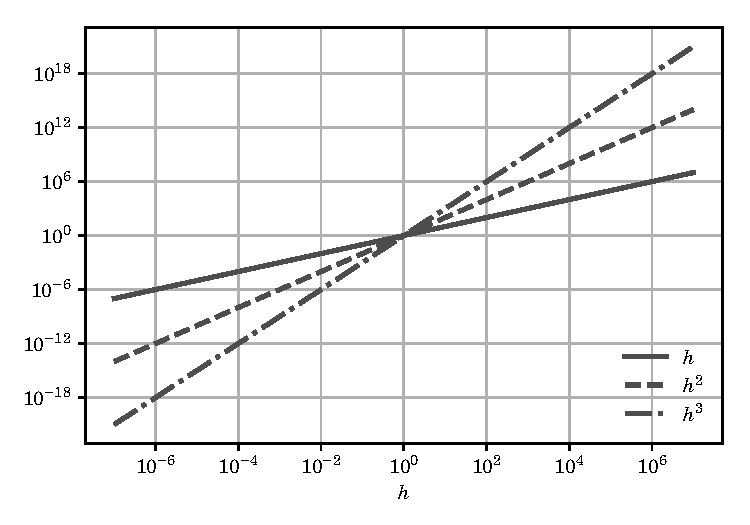
\includegraphics[width=1.0\linewidth]{images/appendix/taylor_example.pdf}
  \caption[Taylor series perturbation]{Behavior of the Taylor coefficients as $h$ decreases.  It is common to refer to the truncated Taylor series which does not include the $h^n$ terms as the \emph{$\mathrm{n}$th-order-Taylor-series approximation} which is clearly only accurate for $h \ll 1$.}
  \label{taylor_perturbations}
\end{figure}

\index{Chain rule of differentiation}
\index{Total derivative}
Assuming that $\rankone{h} = \rankone{r}$ where $\rankone{r}$ is the right-angle vector
\begin{align*}
  \rankone{r} = \{u_i \in \rankone{u} \in \R^n \ |\ u_i = \Vert \rankone{u} \Vert \}
\end{align*}
and noting the fact that $\rankone{r}$ possesses the unique property that $\hat{r} = \rankone{1} = [1\ 1\ \cdots\ 1]\T$, Definition \ref{directional_derivative} in this case yields
\begin{align*}
  \nabla_{\hat{\rankone{r}}} f(\rankone{x}) = \nabla f(\rankone{x}) \cdot \rankone{1} = \parder{f}{x_1} + \parder{f}{x_2} + \cdots + \parder{f}{x_n} = \nabla \cdot \left( f(\rankone{x}) \rankone{1} \right).
\end{align*}
Additionally, in the case that $\rankone{x} = \rankone{x}(t)$ for some $t \in \R$, the chain rule applied to this relation produces the following definition:
\begin{definition}[Total derivative]
\label{total_derivative}
Let $f$ be a function composed of $n$ coordinates of the vector $\rankone{x} = \rankone{x}(t) \in \R^n$ each dependent on a variable $t \in \R$.
The \emph{total derivative} of $f$ with respect to $t$ is
\begin{align*}
  \totder{f}{t} = \parder{f}{x_1}\totder{x_1}{t} + \parder{f}{x_2}\totder{x_2}{t} + \cdots + \parder{f}{x_n}\totder{x_n}{t}.
\end{align*}
\end{definition}

The total derivative is widely used in the field of continuum mechanics, which specifies a variable $f = f(h,t)$ in the \emph{Eulerian frame} of reference defined at a distance $h = h(\rankone{x}, t) = \Vert \rankone{x}(t) - \rankone{x}_0 \Vert$ at time $t$ from an initial coordinate vector $\rankone{x}_0 = \left[ x_0\ y_0\ z_0 \right]\T$ --- referred to as the \emph{Lagrangian frame} --- to the current coordinate vector $\rankone{x}(t) = \left[ x(t)\ y(t)\ z(t) \right]\T$.
On application of the chain rule, the total derivative of the function $f$ with respect to $t$ is given in this case by
\begin{align*}
  \totder{f}{t} \hspace{2mm} \equiv \dot{f} = \hspace{2mm} \parder{f}{t} \totder{t}{t} + \parder{f}{h} \parder{h}{\rankone{x}} \totder{\rankone{x}}{t}
  \hspace{2mm} = \hspace{2mm} \parder{f}{t} + \parder{f}{\rankone{x}} \totder{\rankone{x}}{t},
\end{align*}
which combined with the respective definition of the scalar gradient
\begin{align}
  \label{gradient}
  \parder{f}{\rankone{x}} &\equiv \nabla f = \left[ \parder{f}{x}\ \parder{f}{y}\ \parder{f}{z} \right]\T
\end{align}
and velocity vector
\begin{align}
  \label{velocity}
  \totder{\rankone{x}}{t} &\equiv \rankone{u} = \left[ \totder{x}{t}\ \totder{y}{t}\ \totder{z}{t} \right]\T,
\end{align}
produces
\begin{align}
  \label{material_derivative}
  \dot{f} &= \parder{f}{t} + \rankone{u} \cdot \nabla f.
\end{align}
This quantity has been used often enough that it has been given many other names, including the \emph{material-, convective-, Lagrangian-,} or \emph{substantial-derivative}, among others.
\index{Advection}
The literature commonly refers to the second term $\rankone{u} \cdot \nabla f$ as the \emph{advective} component.
Finally, the overhead-dot notation $(\ \dot{ }\ )$ was first used by \citet{newton_1704} to denote differentiation with respect to time.

\begin{corollary}
\label{functional_taylors_theorem}
An infinitely differentiable functional $\mathcal{J} : A \rightarrow \R$ defined on $A \subseteq V$ with normed linear space $V$ may be expressed as the infinite \textbf{\emph{functional Taylor series}}
\begin{align}
  \label{functional_taylor_series}
  \mathcal{J}(x + \varepsilon h) &= \mathcal{J}(x) + \mathcal{J}'(x) \varepsilon h + \frac{1}{2!} \mathcal{J}''(x) \left( \varepsilon h \right)^2 + \cdots \hspace{2mm},
\end{align}
with $\varepsilon \in \R$ and where $\mathcal{J}'(x)$ is the \textbf{\emph{Gate\^{a}ux derivative}} of the functional $\mathcal{J}$ with respect to its coordinate $x \in A$ in the direction $h \in A$.
\end{corollary}

%%==============================================================================
\section{Mean value theorem} \label{ssn_mean_value_theorem}

\index{Mean value theorem!Definition}
\begin{theorem}[Mean value theorem]
\label{mean_value_theorem}
If the function $f(x)$ is continuous within the closed interval $[a,b] \subset x \in \R$ and is at least once differentiable on the open interval $(a,b)$, there exists a constant $c \in (a,b)$ such that 
\begin{align*}
  \left. \totder{}{x} f(x) \right|_c = \frac{f(a+h) - f(a)}{h},
\end{align*}
where $h = b - a \neq 0$.
\end{theorem}

%%==============================================================================
\section{Fundamental theorem of algebra}

\index{Fundamental theorem of algebra}
\begin{theorem}[Fundamental theorem of algebra]
\label{fundamental_theorem_of_algebra}
Every polynomial equation of degree one or greater has at least one complex root. 
\end{theorem}

%%==============================================================================
\section{Fundamental theorems of calculus}

\begin{theorem}[First fundamental theorem of calculus]
\label{first_fundamental_theorem_of_calculus}
\index{Fundamental theorems of calculus!First theorem}
First, if a given function $f(x)$ is continuous within a closed interval $[a,b]$ and $F(x)$ is the anti-derivative or indefinite integral of $f(x)$, then
\begin{align*}
  \int_a^b f(x) \d{x} = F(b) - F(a).
\end{align*}
\end{theorem}

\begin{theorem}[Second fundamental theorem of calculus]
\label{second_fundamental_theorem_of_calculus}
\index{Fundamental theorems of calculus!Second theorem}
Second, if $f(x)$ is a continuous function within an open interval $(a,b)$, the anti-derivative or indefinite integral $F(x)$ is defined as
\begin{align*}
  F(x) = \int_a^x f(t) \d{t} \hspace{5mm} \text{with inverse} \hspace{5mm} 
  \totder{F}{x} = f(x)
\end{align*}
at each point in $x \in (a,b)$.
\end{theorem}

%%==============================================================================
\section{Fundamental lemma of calculus of variations}

\begin{lemma}[Fundamental lemma of calculus of variations]
\index{Fundamental lemma of calculus of variations}
\label{fundamental_lemma}
If $f(x)$ is continuous over the domain $\Omega(x) \subset \R^n$ and if
\begin{align*}
  \int_{\Omega} f(x) h(x) \d{\Omega} = 0
\end{align*}
for all compactly supported functions $h(x)$, then $f(x) \equiv 0$.
\end{lemma}

%%==============================================================================
\section{Divergence identities} \label{ssn_divergence_identities}

For rank-one tensors $\rankone{u}$, $\rankone{w}$ and scalar $\phi$, the following identities follow by linearity of the divergence operator:
\begin{align}
  \label{divergence_identity_1}
  \nabla \cdot \left( \phi \rankone{u} \right) &= \rankone{u} \cdot \nabla \phi + \phi \nabla \cdot \rankone{u}  \\
  \nabla \cdot \left( \phi \rankone{u} \rankone{w} \right) &= \rankone{u} \rankone{w} \cdot \nabla \phi + \phi \nabla \cdot \left( \rankone{u} \rankone{w} \right) \notag \\
  \label{divergence_identity_2}
  &= \rankone{u} \rankone{w} \cdot \nabla \phi + \phi \left( \rankone{w} \nabla \cdot \rankone{u} + \rankone{u} \cdot \nabla \rankone{w} \right) \\
  \label{divergence_identity_3}
  \nabla \cdot \left( \rankone{u} \rankone{w} \right) &= \rankone{u} \cdot \nabla \rankone{w} + \rankone{w} \nabla \cdot \rankone{u}.
\end{align}

%%==============================================================================
\section{Dyadic product}

\begin{definition}
\index{Dyad, Outer product} 
For rank-one tensors $\rankone{u}$ and $\rankone{n}$, the \emph{dyadic product}, or \emph{outer product} of $\rankone{u}$ and $\rankone{n}$ is given by
\begin{align*}
  \rankone{u} \rankone{n} =
    \begin{bmatrix}
      u n_x & u n_y & u n_z \\
      v n_x & v n_y & v n_z \\
      w n_x & w n_y & w n_z
    \end{bmatrix}.
\end{align*}
\end{definition}

\begin{remark}
\label{dydadic_unit_vector_product}
In particular, if $\rankone{n}$ is a unit vector,
\begin{align*}
  \rankone{u} \rankone{n} \cdot \rankone{n} =
    \begin{bmatrix}
      u n_x^2 + u n_y^2 + u n_z^2 \\
      v n_x^2 + v n_y^2 + v n_z^2 \\
      w n_x^2 + w n_y^2 + w n_z^2
    \end{bmatrix} = 
    \begin{bmatrix}
      u \rankone{n} \cdot \rankone{n} \\
      v \rankone{n} \cdot \rankone{n} \\
      w \rankone{n} \cdot \rankone{n}
    \end{bmatrix}
    = \rankone{u},
\end{align*}
\begin{align*}
  \rankone{n} \rankone{n} =
    \begin{bmatrix}
      n_x n_x & n_x n_y & n_x n_z \\
      n_y n_x & n_y n_y & n_y n_z \\
      n_z n_x & n_z n_y & n_z n_z
    \end{bmatrix}.
\end{align*}
\end{remark}

%%==============================================================================
\section{Divergence theorem} \label{ssn_divergence_theorem}

The following important theorem was likely first stated by \citet{lagrange_1762}.

\begin{theorem}[Divergence theorem]
\index{Divergence theorem!Definition}
\label{divergence_theorem}
The integral of the divergence of a continuously-differentiable vector field $\rankone{j}$ inside a open, bounded volume $\Omega$ is equal to the integral of the outward flux of the vector field across the surface of the volume $\Gamma$:
\begin{align*}
  \int_{\Gamma} \rankone{j} \cdot \rankone{n} \d{\Gamma} = \int_{\Omega} \nabla \cdot \rankone{j} \d{\Omega}.
\end{align*}
The proof of this may be found in any multi-dimensional calculus textbook.
\end{theorem}

%%==============================================================================
\section{Leibniz's rule} \label{ssn_liebniz_rule}

\index{Leibniz's rule!Definition}
\begin{theorem}[Leibniz's rule]
\label{leibniz_rule}
Leibniz formula, referred to as \textbf{\emph{Leibniz's rule for differentiating an integral with respect to a parameter that appears in the integrand and in the limits of integration}}, states that
\begin{align*}
  \totder{}{x} \int_{a(x)}^{b(x)} f(x,y) \d{y} = &+ \int_{a(x)}^{b(x)} f_x(x,y) \d{y} \notag \\
  &+ f(x,b(x)) \totder{b}{x} - f(x,a(x))\totder{a}{x},
\end{align*}
where $f(x,y)$ and $f_x(x,y)$ are both continuous over the finite domain $y \in [a(x),b(x)]$.
\end{theorem}

\begin{proof}
Let
$$I(x,a(x),b(x)) = \totder{}{x} \int_{a(x)}^{b(x)} f(x,y) \d{y}.$$
Using Definition \ref{total_derivative}, the total derivative of $I$ with respect to $x$ is
$$\totder{I}{x} = \parder{I}{x} \totder{x}{x} + \parder{I}{a} \totder{a}{x} + \parder{I}{b} \totder{b}{x}.$$
Next, due to the fact that integration is performed over the coordinate $y$, the linear operations of partial $x$-differentiation and integration over $y$ may be safely exchanged.
Therefore,
\begin{align*}
  \parder{I}{x} &= \parder{}{x} \int_{a(x)}^{b(x)} f(x,y) \d{y} = \int_{a(x)}^{b(x)} f_x(x,y) \d{y}.
\end{align*}
Next, using Definition \ref{first_fundamental_theorem_of_calculus}, if $F(x,y)$ is the indefinite integral of $f(x,y)$ with respect to $y$ on $y \in [a,b]$,
\begin{align*}
  \parder{I}{a} &= \parder{}{a} \int_{a(x)}^{b(x)} f(x,y) \d{y} \\
                &= \parder{}{a} \Big[ F(x,b(x)) - F(x,a(x)) \Big] = - f(x,a(x)).
\end{align*}
Likewise,
\begin{align*}
  \parder{I}{b} &= \parder{}{b} \int_{a(x)}^{b(x)} f(x,y) \d{y} \\
                &= \parder{}{b} \Big[ F(x,b(x)) - F(x,a(x)) \Big] = f(x,b(x)).
\end{align*}
Therefore, combining the above relations results in
$$\totder{I}{x} = \int_{a(x)}^{b(x)} f_x(x,y) \d{y} + f(x,b(x))\totder{b}{x} - f(x,a(x))\totder{a}{x}.$$
\end{proof}

%%==============================================================================
\section{Outward-pointing-unit-normal vector} \label{ssn_normal_vector}
\index{Unit-normal vector}

Consider a fixed body $\Omega(\rankone{x})$ with intrinsically-defined upper surface $\Gamma_{\srf}(\rankone{x}) = z - S(x,y)$ and lower surface $\Gamma_{\bed}(\rankone{x}) = B(x,y) - z$.
It follows that the gradient of the upper and lower surface is given by
\begin{align*}
  \nabla \Gamma_{\srf}(\rankone{x}) = \rankone{\hat{k}} - \nabla S(x,y)
  \hspace{5mm} \text{and} \hspace{5mm}
  \nabla \Gamma_{\bed}(\rankone{x}) = \nabla B(x,y) - \rankone{\hat{k}},
\end{align*}
where $\rankone{\hat{k}}$ us the unit-vector pointing in the direction of the $z$ coordinate.
The \emph{outward-pointing-unit-normal vector} is simply the normalized version of these vectors, respectively 
\begin{align*}
  \left. \rankone{n} \right|_{\Gamma_S} = \frac{ \nabla \Gamma_{\srf}(\rankone{x}) }{\Vert \nabla \Gamma_{\srf}(\rankone{x}) \Vert},
  \hspace{10mm} \text{and} \hspace{10mm}
  \left. \rankone{n} \right|_{\Gamma_B} = \frac{ \nabla \Gamma_{\bed}(\rankone{x}) }{\Vert \nabla \Gamma_{\bed}(\rankone{x}) \Vert}
\end{align*}
with gradient magnitudes given by the $L^2$ norm
\begin{align*}
  \Vert \nabla \Gamma_{\srf}(\rankone{x}) \Vert &= \left( \rankone{\hat{k}} \cdot \rankone{\hat{k}} - 2 \rankone{\hat{k}} \cdot \nabla S + \nabla S \cdot \nabla S \right)^{\frac{1}{2}} \\
                                                &= \left( 1 - 2 \parder{S}{z} + \nabla S \cdot \nabla S \right)^{\frac{1}{2}} = \left( 1 + \nabla S \cdot \nabla S \right)^{\frac{1}{2}} \\ 
  \Vert \nabla \Gamma_{\bed}(\rankone{x}) \Vert &= \left( \nabla B \cdot \nabla B - 2 \rankone{\hat{k}} \cdot \nabla B + \rankone{\hat{k}} \cdot \rankone{\hat{k}} \right)^{\frac{1}{2}} \\
                                                &= \left( \nabla B \cdot \nabla B - 2 \parder{B}{z} + 1 \right)^{\frac{1}{2}} = \left( \nabla B \cdot \nabla B + 1 \right)^{\frac{1}{2}},
\end{align*}
where $\partial_z S = \partial_z B = 0$ has been used.

%%==============================================================================
\section{Reynolds transport theorem} \label{ssn_reynolds_transport_theorem}

\begin{theorem}[Reynolds transport theorem]
\label{reynolds_transport_theorem}
Within an arbitrary time-evolving volume $\Omega(t) \in \R^3$ with boundary $\Gamma(t)$ moving with the flow of a fluid, \emph{Leibniz's rule in three dimensions} -- better known in continuum mechanics as \index{Reynolds transport theorem} \textbf{\emph{Reynolds transport theorem}} \citep{reynolds_1903} -- states that for a given quantity $\phi$,
\begin{align*}
  \totder{}{t} \int_{\Omega(t)} \phi \d{\Omega}(t) = \int_{\Omega(t)} \parder{\phi}{t} \d{\Omega(t)} + \int_{\Gamma(t)} \phi \rankone{w} \cdot \rankone{n} \d{\Gamma(t)},
\end{align*}
where $\rankone{w}$ is the velocity of surface $\Gamma(t)$ due to changes in $\Omega(t)$ and $\rankone{n}$ is the outward-facing unit-normal vector for $\Gamma(t)$.
\end{theorem}

\begin{corollary}
\label{constant_volume_reynolds}
If the volume remains constant, \ie, $\Omega \neq \Omega(t), \Gamma \neq \Gamma(t)$, $\rankone{w} \cdot \rankone{n} = 0$, and Theorem (\ref{reynolds_transport_theorem}) reduces to
\begin{align*}
  \totder{}{t} \int_{\Omega} \phi \d{\Omega} = \int_{\Omega} \parder{\phi}{t} \d{\Omega}.
\end{align*}
\end{corollary}

%%==============================================================================
\section{Continuity equations} \label{ssn_continuity_equations}

Within a arbitrary fixed volume $\Omega$ with boundary $\Gamma$, 
\begin{align*}
  \begin{matrix}
    \text{the total} \\
    \text{rate of change} \\
    \text{of quantity $\phi$} \\
    \text{in $\Omega$}
  \end{matrix} \hspace{2.5mm} = \hspace{2.5mm} 
  \begin{matrix}
    \text{the inward flux} \\
    \text{of $\phi$ across the} \\
    \text{boundary $\Gamma$} \\
  \end{matrix} \hspace{2.5mm} + \hspace{2.5mm} 
  \begin{matrix}
    \text{the generation} \\
    \text{of quantity $\phi$} \\
    \text{within $\Omega$}
  \end{matrix}, 
\end{align*}
or mathematically, the integral form of the \emph{continuity equation}
\begin{align}
  \label{integral_continuity_equation}
  \totder{}{t} \int_{\Omega} \phi \d{\Omega} \hspace{2.5mm} = \hspace{2.5mm} - \int_{\Gamma} \left( \phi \rankone{u} + \rankone{j} \right) \cdot \rankone{n} \d{\Gamma} \hspace{2.5mm} + \hspace{2.5mm} \int_{\Omega} \mathring{f} \d{\Omega},
\end{align}
with source term $\mathring{f}$, material velocity $\rankone{u}$, advective flux $\phi \rankone{u}$, non-advective flux $\rankone{j}$, and outward-pointing unit-normal-vector $\rankone{n}$.  Applying Reynolds transport theorem corollary (\ref{constant_volume_reynolds}) to the total time derivative and divergence theorem (\ref{divergence_theorem}) \index{Divergence theorem!Regarding continuity equations} to the surface integral,
\begin{align*}
  \int_{\Omega} \parder{\phi}{t} \d{\Omega} + \int_{\Omega} \nabla \cdot \left( \phi \rankone{u} + \rankone{j} \right) \d{\Omega} &= \int_{\Omega} \mathring{f} \d{\Omega}.
\end{align*}
Therefore, because the integral was taken arbitrarily, the \emph{differential form} of the continuity equation is
\begin{align}
  \label{differential_continuity_equation}
  \parder{\phi}{t} + \nabla \cdot \left( \phi \rankone{u} + \rankone{j} \right) = \mathring{f}.
\end{align}
The advective-flux divergence term can be expanded:
\begin{align*}
  \parder{\phi}{t} + \rankone{u} \cdot \nabla \phi + \phi \nabla \cdot \rankone{u} + \nabla \cdot \rankone{j} = \mathring{f},
\end{align*}
which can be reducing using total derivative (\ref{total_derivative}) to 
\begin{align}
  \label{nonconservative_continuity_equation}
  \totder{\phi}{t} + \phi \nabla \cdot \rankone{u} + \nabla \cdot \rankone{j} = \mathring{f}.
\end{align}
Equations (\ref{differential_continuity_equation}) and (\ref{nonconservative_continuity_equation}) are respectively referred to as the \emph{conservative} and \emph{non-conservative} forms of the continuity equation \citep{anderson_1995}.

%%==============================================================================
\section{Conservation equations} \label{ssn_conservation_equations}

First, conservation of mass begins from continuity equation (\ref{differential_continuity_equation}) with $\phi = \rho$, $\rankone{j} = \rankone{0}$, and $\mathring{f} = \mathring{\rho}$,
\begin{align*}
  \parder{\rho}{t} + \nabla \cdot \left( \rho \rankone{u} \right) = \mathring{\rho}& && \leftarrow \text{continuity equation} \\ 
  \parder{\rho}{t} + \rankone{u} \cdot \nabla \rho + \rho \nabla \cdot \rankone{u} = \mathring{\rho}& && \leftarrow \text{divergence identity} \\ 
  \totder{\rho}{t} + \rho \nabla \cdot \rankone{u} = \mathring{\rho}& && \leftarrow \text{chain rule with $\rankone{u} = \dot{\rankone{x}}$, $\dot{t} = 1$}.
\end{align*}
Using the definition of density $\rho = m/V$ with mass $m$ and volume $V$,
\begin{align*}
  \frac{\dot{m}V - \dot{V}m}{V^2} + \frac{m}{V} \nabla \cdot \rankone{u} &= \frac{\mathring{m}}{V} && \leftarrow \text{quotient rule} \\
  \frac{\dot{m}}{m} - \frac{\dot{V}}{V} + \nabla \cdot \rankone{u} &= \frac{\mathring{m}}{m} && \leftarrow \text{algebra} \\
  \frac{1}{V} \totder{V}{t} &= \nabla \cdot \rankone{u} && \leftarrow \text{$\mathring{m} = \dot{m}$}.
\end{align*}
The equality used to derived the final expression is equivalent to the Eulerian expression
\begin{align*}
  \parder{m}{t} + \rankone{u} \cdot \big( \nabla m \big) = \mathring{m}.
\end{align*}
Therefore, the system of two Eulerian equations for $m$ and $V$ are respectively
\begin{align*}
  \parder{V}{t} + \rankone{u} \cdot \big( \nabla V \big) = V \nabla \cdot \rankone{u}, \hspace{10mm} 
  \parder{m}{t} + \rankone{u} \cdot \big( \nabla m \big) = \mathring{m},
\end{align*}
and are consistent with the Lagrangian equations 
\begin{align*}
  \totder{V}{t} = V \nabla \cdot \rankone{u}, \hspace{10mm}
  \totder{m}{t} = \mathring{m}.
\end{align*}

%%==============================================================================
\section{Finite-volume method} \label{ssn_finite_volume_method}

\index{Finite-volume method}
Let $V$ be the volume of the domain $\Omega$ and $\bar{g} = V^{-1} \int_{\Omega} g \d{\Omega}$ be the volume average of a measurable quantity $g(x,t)$.
Integral continuity equation (\ref{integral_continuity_equation}) may be represented exactly as
\begin{align}
  \label{finite_volume_continuity}
  V \totder{\bar{\phi}}{t} + \int_{\Gamma} \left( \phi \rankone{u} + \rankone{j} \right) \cdot \rankone{n} \d{\Gamma} &= V \bar{\mathring{f}}.
\end{align}
This is the fundamental equation from which the class of numerical approximation methods termed \emph{finite-volume methods} emerged.
These methods produce a local approximation of the average of a quantity over finite cells, and require a specification of the non-advective-cell flux $\rankone{j}$.
Note that similar to the derivation of continuity equation (\ref{differential_continuity_equation}), the surface integral may be converted to a volume integral using divergence theorem (\ref{divergence_theorem}),
\begin{align}
  \label{finite_volume_continuity}
  V \totder{\bar{\phi}}{t} + \int_{\Omega} \nabla \cdot \left( \rho \rankone{u} + \rankone{j} \right) \d{\Omega} &= V \bar{\mathring{f}}.
\end{align}

%%==============================================================================
\section{The inverse problem of the calculus of variations}

\begin{definition}
\index{Variational principle}
For non-conservative systems, the Lagrangian $\mathscr{L}$ cannot be determined from the equations of motion; this is because there is no closed-form equation for the potential energy.
The \emph{inverse problem} is to determine $\mathscr{L}$ such that
\begin{align*}
  \delta \int_t \mathscr{L} \d{t} = 0.
\end{align*}
The $\mathscr{L}$ satisfying this \emph{variational principle} corresponds with the Euler-Lagrange equations --- the equations of motion --- of the system.
\end{definition}
